\chapter{Beispiele von Verfahren}

\section{K-means}
K-means ist ein Clustering Algorithmus und somit ein unsupervised Verfahren. Das Ziel ist es Daten zu Gruppieren, die nicht vorher mit einem Label versehen wurden.

Der Trainingsschritt besteht daraus, die Trainingsdaten in K Gruppen oder eben Cluster zu verteilen. Anschliessend können wir dem trainierten Modell ein Datensatz füttern und erhalten als Resultat den zugehörigen Cluster.

Als Beispiel können wir hier wieder Netflix zur Hand nehmen. Netflix kann mittels K-means seine Nutzenden in eine beliebige Anzahl Cluster einteilen lassen. Dieser Trainingsschritt kann mittels den bestehenden Benutzerdaten gemacht werden. Meldet sich nun eine weitere Person an, kann diese aufgrund seiner Daten anschliessend einer dieser Gruppen zugewiesen werden. Somit kann Netflix dieser Person Vorschläge machen, die auf diesem Cluster basieren. Haben als Beispiel 80\% der Nutzenden aus diesem Cluster den Film <<the social dilemma>> gesehen, schlagen wir diesen Film vor.

\subsection{K in K-means}
Das K in K-means gibt dabei vor, wie viele Cluster wir generieren wollen. Dieser Wert K wird durch die Person definiert, die den Algorithmus trainiert und nicht vom Algorithmus selber. Somit nennt sich K ein Hyperparameter. Hyperparameter sind alle Konfigurationen die vor dem Training durch den Menschen bestimmt werden und nicht durch den Algorithmus.

\subsection{Funktionsweise}
K-Means arbeitet mit sogenannten Zentroiden. Dabei gibt es pro Cluster einen Zentroiden. Dieser Zentroiden ist der Mittelpunkt des Clusters. Die Distanz zwischen zwei Punkten kann mittels der euklidischen Distanz berechnet werden.
Der Zentroiden ist anschliessend der Wert mit den im Schnitt kleinsten euklidischen Abstand zu jedem Element im Cluster.

Der Ablauf von K-Means lässt sich also folgendermassen zusammenfassen:
\begin{enumerate}
	\item Zuerst bestimmen wir K zufällige Zentroiden
	\item Jeder Datenwert wird nun dem nächstliegenden Zentroiden zugewiesen. Dadurch werden alle Elemente eindeutig einem Cluster zugewiesen.
	\item Nun berechnen wir pro Cluster den Zentroiden neu, damit dieser möglichst einen kleinen Abstand zu allen Elementen im Cluster hat.
	\item Durch die Verschiebung der Zentroiden ist es nun möglich, dass ein Datensatz nicht mehr im Cluster mit dem nächstgelegenen Zentroiden ist. Deshalb führen wir die Schritte 2 und 3 solange aus, bis bei einem Durchgang kein Datensatz mehr den Cluster wechselt. Es können auch andere Abbruchbedingungen definiert werden, wie zum Beispiel eine maximale Anzahl an Durchgängen.
\end{enumerate}

\subsection{Bemerkungen}
\begin{itemize}
	\item K muss bereits vor Beginn des Trainings definiert werden. Diese Wahl ist somit essenziell für die Zugehörigkeit eines Elementes zu einer Gruppe. Es gibt verschiedene Techniken, die Qualität von den Clustern unter verschiedenen K zu prüfen. Zwei davon sind die Elbow-Methode und der Silhouettenkoeffizient.
	\item Ebenfalls relevant für die Qualität der Cluster ist die initiale Platzierung der Zentroiden. Je nach Platzierung können mit denselben Daten andere Cluster entstehen. Auch hier gibt es hilfreiche Algorithmen, wie k-means++. Bei k-means++ werden die Zentroiden so weit voneinander wie möglich platziert, was zu besseren Resultaten führt als die komplett zufällige Platzierung.
\end{itemize}

\subsection{Notebook}
Im Internet finden sich viele gute Python Notebooks zu K-means. Einen guten Überblick über K-means findet sich als Beispiel hier:

\url{https://colab.research.google.com/github/jakevdp/PythonDataScienceHandbook/blob/master/notebooks/05.11-K-Means.ipynb}

\subsection{Beispiel}
\begin{figure}[h!]
	\centering
	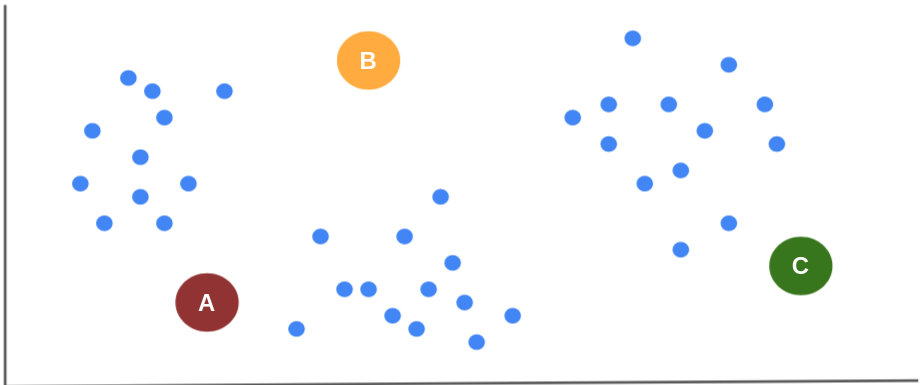
\includegraphics[width=0.8\textwidth]{kmeans1.png}
	\caption{Initiale Platzierung der Zentroiden (Quelle: Eigenkreation)}
\end{figure}

\begin{figure}[h!]
	\centering
	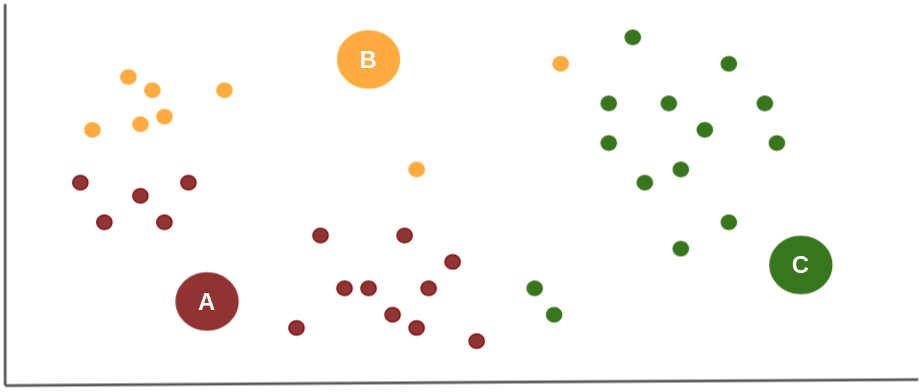
\includegraphics[width=0.8\textwidth]{kmeans2.png}
	\caption{Zuweisen der Elemente zum nächsten Zentroiden (Quelle: Eigenkreation)}
\end{figure}

\begin{figure}[h!]
	\centering
	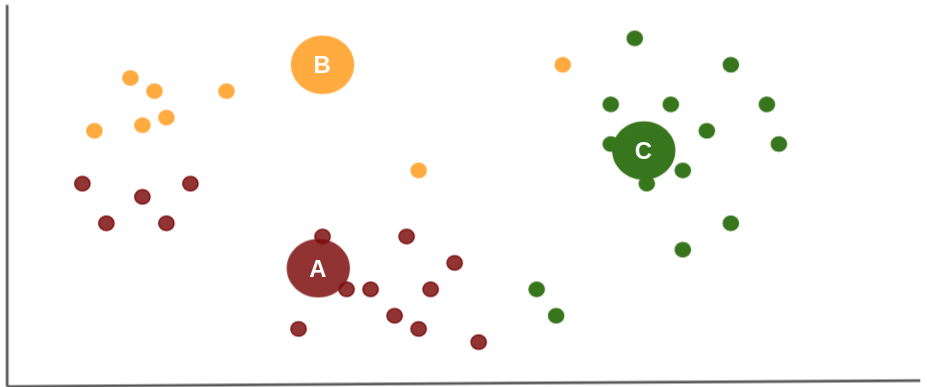
\includegraphics[width=0.8\textwidth]{kmeans3.png}
	\caption{Neuplatzierung der Zentroiden (Quelle: Eigenkreation)}
\end{figure}

\begin{figure}[h!]
	\centering
	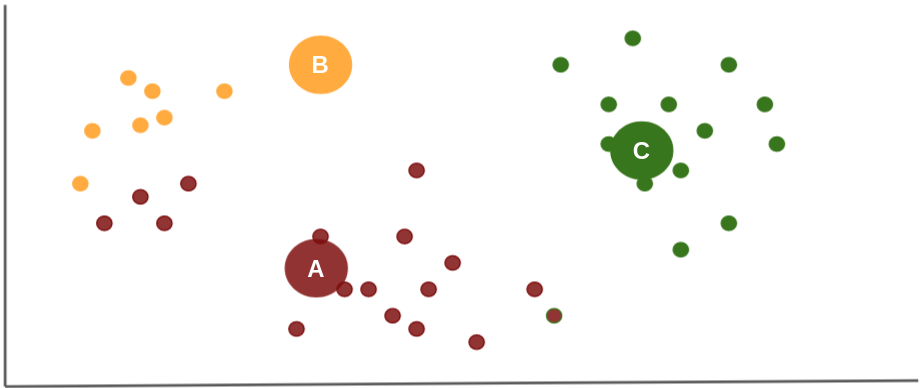
\includegraphics[width=0.8\textwidth]{kmeans4.png}
	\caption{Neue Zuweisung der Elemente zum nächsten Zentroiden (Quelle: Eigenkreation)}
\end{figure}

\begin{figure}[h!]
	\centering
	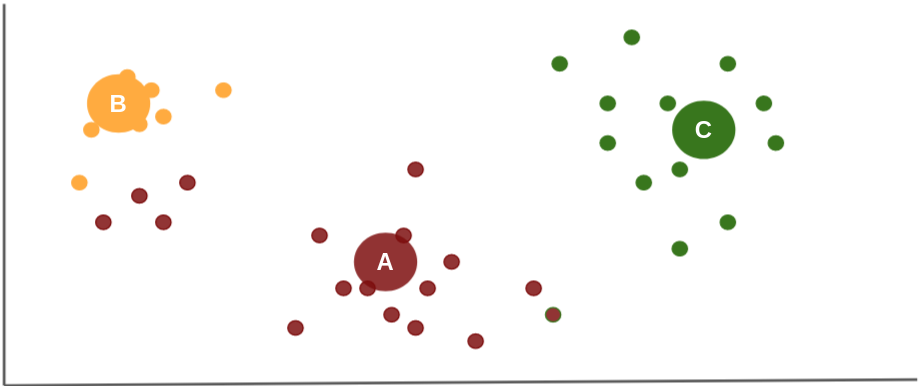
\includegraphics[width=0.8\textwidth]{kmeans5.png}
	\caption{Erneute Neuplatzierung der Zentroiden (Quelle: Eigenkreation)}
\end{figure}

\begin{figure}[h!]
	\centering
	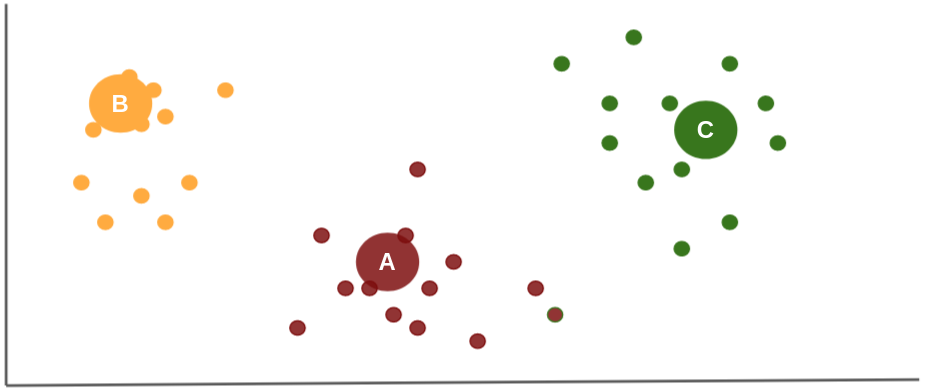
\includegraphics[width=0.8\textwidth]{kmeans6.png}
	\caption{Neue Zuweisung der Elemente zum nächsten Zentroiden (Quelle: Eigenkreation)}
\end{figure}

\begin{figure}[h!]
	\centering
	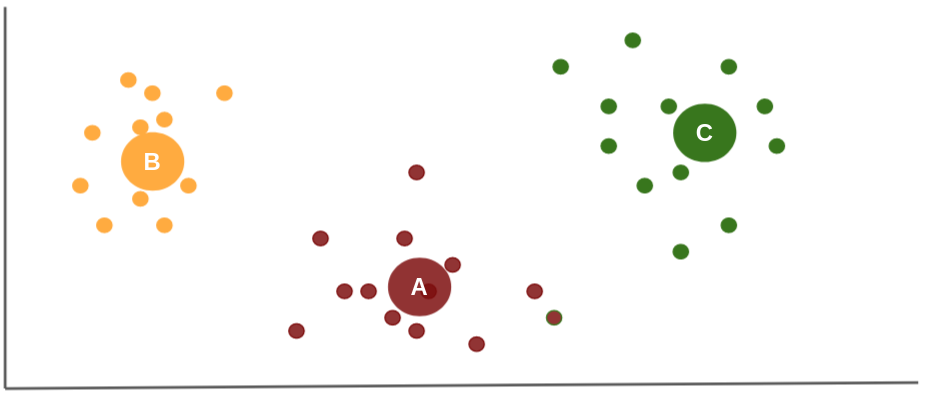
\includegraphics[width=0.8\textwidth]{kmeans7.png}
	\caption{Sobald es keine Verschiebung mehr gibt, sind wir fertig (Quelle: Eigenkreation)}
\end{figure}

\clearpage
\section{Random Forest}
\subsection{Decision Tree}
Damit das Konzept von Random Forest erläutert werden kann, muss zuerst das Konzept eines Decision Tree (Entscheidungsbaum) erläutert werden. 
Ein Decision Tree kann für die Klassifizierung oder eine Regression verwendet werden. In unserem Beispiel verwenden wir den Decision Tree für die Klassifizierung von Datensätzen.

\begin{figure}[h!]
	\centering
	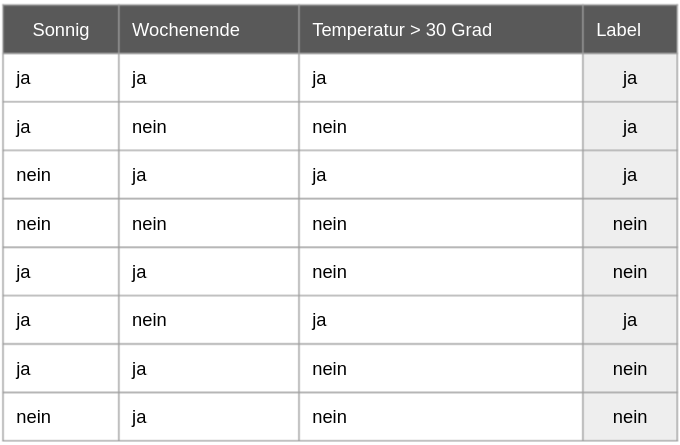
\includegraphics[width=0.8\textwidth]{decision-tree.png}
	\caption{Trainingsdaten (Quelle: Eigenkreation)}
\end{figure}

In diesem Beispiel haben wir Datensätze, bei welchen jeweils angegeben ist, ob es an einem Tag sonnig war, ob es über 30 Grad warm war und ob es sich um einen Samstag oder Sonntag (Wochenende) gehandelt hat. In der Spalte <Label> ist angegeben, ob eine Person an diesem Tag in die Aare gesprungen ist oder nicht.

Aus diesen Daten wollen wir nun einen Decision Tree erstellen. Dafür wird nacheinander eines der Attribute (<Sonnig>, <Wochenende>, <Temperatur>) genommen und die Datensätze nach diesem Attribut getrennt. In welcher Reihenfolge wir die Attribute abarbeiten können wir mittels verschiedenen Methoden bestimmen. Das Ziel davon ist jeweils, nach der Aufteilung durch das Attribut möglichst alle Elemente mit <Label> ja auf einer Seite zu haben und alle anderen auf der anderen Seite. Zwei gängige Verfahren sind die Berechnung der Entropie oder des Gini-Faktors. In unserem Beispiel würde der Baum dann so aussehen:
\clearpage
\begin{figure}[h!]
	\centering
	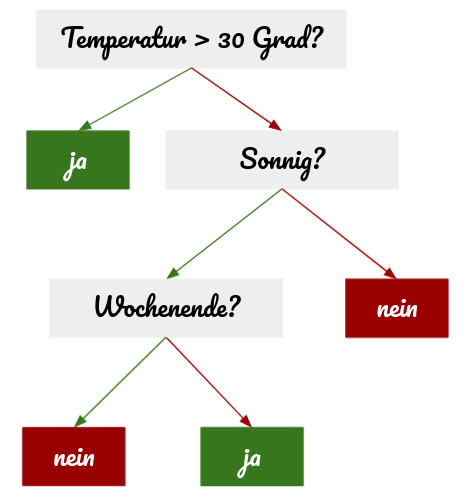
\includegraphics[width=0.4\textwidth]{decision-tree2.png}
	\caption{Trainingsdaten (Quelle: Eigenkreation)}
\end{figure}
Erläuterung zur Grafik: Hier wurde zuerst nach der Temperatur gefragt, da alle Datensätz mit einer Temperatur von über 30 Grad dem Label <Ja> zugeordnet werden können. Somit haben wir auf der linken Seite nur noch Datensätze mit dem Label <Ja>. Auf der rechten Seite fragen wir uns nun, ob es sonnig war. Bei allen nun übrig gebliebenen Datensätzen bei denen dies nicht zutrifft, lautet das Label <Nein>. Somit bleibt uns als letzte Frage das Wochenende. Bei allen übrig gebliebenen Datensätzen, an denen Wochenende war, lautet das Label <Nein>.

Das Problem bei solchen Decision Trees ist, dass sie sehr schnell overfitted sind. In unserem Beispiel sehen wir, dass alle Testdaten am Ende korrekt zugewiesen werden würden. Allerdings sehen wir auch, dass ein Eintrag, bei dem die Temperatur grösser 30 Grad war, immer zum Label <Ja> führt in unserem Baum. Diese Bedingung muss aber in zukünftigen Daten nicht zwangsläufig gegeben sein. Wir haben also einen Baum erstellt, der perfekt zu den Testdaten, nicht aber zwangsläufig zu weiteren Eingaben passt. Genau dieses Verhalten nennen wir Overfitting.

Anmerkung: Grundsätzlich muss ein Decision Tree nicht alle Testdaten korrekt klassifizieren (meist ist dies auch gar nicht möglich). Hier können wir z. B. angeben, dass wir auch mit 95\% korrekten Klassifizierungen zufrieden sind.
\subsection{Random Forest}
Um das Problem des Overfitting zu beheben, verwenden wir nun anstelle eines Decision Tree einen Random Forest. Ein Random Forest besteht dabei aus mehreren Decision Trees. Dabei haben wir die Möglichkeit bei der Erstellung der einzelnen Trees jeweils nur eine gewisse Anzahl an Daten (Reihen oder Spalten) zu verwenden.
Dadurch werden die einzelnen Bäume auf die gesamte Datenmenge diverser, was unser Overfitting verhindert.

Um anschliessend einen Datensatz zu klassifizieren, lassen wir diesen durch alle Trees in unserem Forest laufen. Anschliessend wählen wir demokratisch das häufigste Resultat als korrekt. 

\begin{figure}[h!]
	\centering
	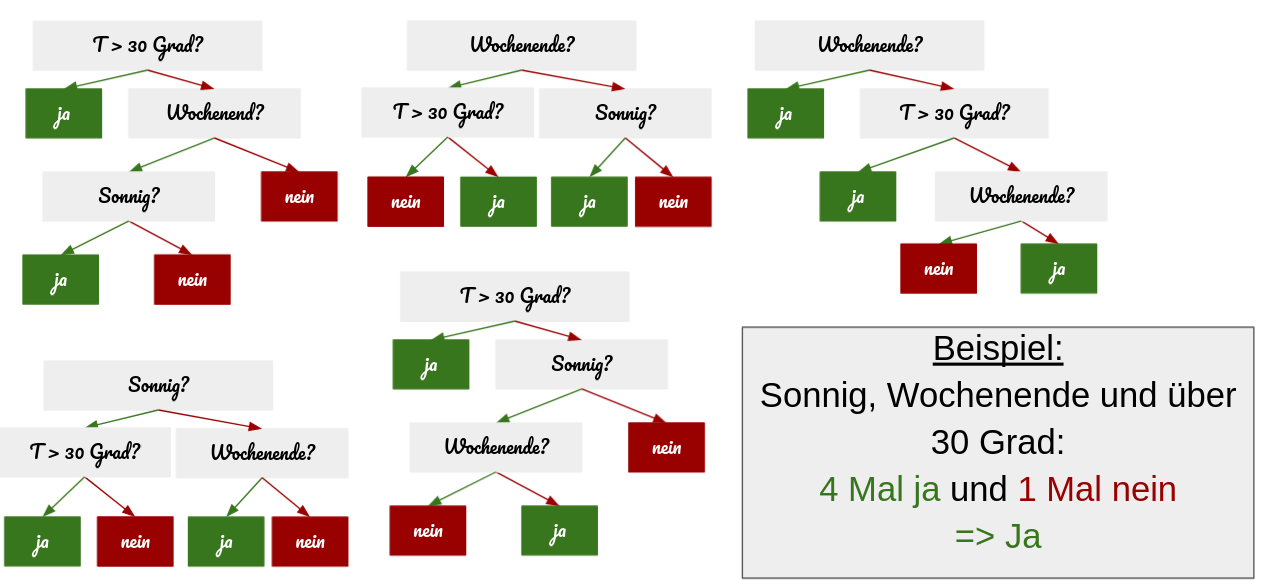
\includegraphics[width=1\textwidth]{forest.png}
	\caption{Random Forest (Quelle: Eigenkreation)}
\end{figure}
Erläuterung zur Grafik: Hier haben wir fünf verschiedene Trees erstellt, indem wir jeweils nur einen Bruchteil der Testdaten für das Training verwendet haben. Deshalb erhalten wir fünf verschiedene Trees. Um nun das korrekte Label zu bestimmen, prüfen wir unseren Datensatz mit allen Trees. In diesem Beispiel ergeben vier Trees ein ja und nur einer ein nein. Deshalb wählen wir als Label das Ja aus.
\subsection{Notebook}
Auch zu Random Forest finden sich viele Beispiele im Internet. Als Einstieg kann folgendes Notebook empfohlen werden: 
\url{https://github.com/WillKoehrsen/Machine-Learning-Projects/blob/master/random_forest_explained/Random\%20Forest\%20Explained.ipynb}
